\chapter{Description microscopique des bois feuillus}\label{feuillus}

\begin{abstract}
Ce chapitre décrit chacun des types de cellules rencontrés chez les arbres feuillus. Nous nous attardons aussi à certaines caractéristiques anatomiques, comme la disposition des cellules de parenchymes longitudinaux, qui permettent d'identifier les espèces.
\end{abstract}

\minitoc

\section{Introduction}

Un certain nombre de différences importantes existent entre la microstructure des bois résineux et celle des bois feuillus. Les principales sont les suivantes :\\

\begin{description}

\item[Les bois feuillus possèdent des cellules spécialisées dans le transport de la sève brute] L'ensemble des éléments de vaisseaux forme les vaisseaux qui sont de véritables conduites servant au transport de la sève brute. Ces vaisseaux sont aussi appelés pores. On peut les voir aisément à l'aide d'une loupe de grossissement $\times$10 chez la plupart des bois feuillus.\\

\item[On ne retrouve pas d'alignement radial net des cellules longitudinales chez les feuillus] Ceci s'explique par la croissance en diamètre très importante des éléments de vaisseaux après leur formation au niveau de l'initiale du cambium, contrairement aux autres cellules longitudinales qui vont s'allonger.  On note également une croissance du cambium ralentie près des éléments de vaisseaux, ce qui favorise la croissance en diamètre de ces derniers. L'absence d'alignement des cellules est mis en évidence par le louvoiement des rayons ligneux lorsqu'on les observe en plan transversal.\\

\item[Les feuillus ont une structure beaucoup plus complexe que celle des résineux] On retrouve un plus grand nombre de types de cellules de même que plus de variation en dimension, forme et disposition des cellules à l'intérieur d'un cerne annuel. \\

\item[Les rayons des bois feuillus sont plus variables en largeur que ceux des bois résineux] En effet, chez les résineux, les rayons sont unisériés dans la grande majorité des cas de sorte qu'on ne peut pas les voir à l'œil nu ou à l'aide d'une loupe de faible grossissement ($\times$10).  Chez les feuillus, les rayons sont beaucoup plus larges (bisériés et jusqu'à 30-sériés et plus) de sorte qu'on utilise leur largeur comme critère d'identification à la loupe. Par exemple, la largeur des rayons est un excellent critère permettant de distinguer les érables durs (\textit{Acer spp.}) des bouleaux (\textit{Betula spp}.). De plus, les rayons des feuillus peuvent contenir plus d'un type de cellules de parenchymes.\\
\end{description}

La liste des différents types de cellules rencontrées dans les bois feuillus est présentée à la figure~\ref{fig:resum_feuillus}. La forme et la dimension relative des principaux types de cellules sont présentées aux Figures~\ref{fig:ch4_type_cell}~et~\ref{fig:ch4_form_cell_X}.  On remarque que les fibres sont les cellules les plus allongées et celles qui possèdent les parois cellulaires les plus épaisses. Ces caractéristiques leurs confèrent la fonction principale de support mécanique de la tige. Chaque type de cellule sera décrit dans les paragraphes qui suivent.

\begin{figure}[h]
\centering

\begin{tikzpicture}[level distance=2.25in,sibling distance=.2in,scale=.75]
\tikzset{edge from parent/.style= 
            {thick, draw,
                edge from parent fork right},every tree node/.style={draw,minimum width=1in,text width=1.5in, align=center},grow'=right}
\Tree 
   [
    [. {Cellules longitudinales}
        [.{Éléments de vaisseaux}
        ]
        [.{Trachéides}
            [.{Vaculaires} ]
            [.{Juxtavasculaires} ]
        ] 
        [. {Fibres}
        	[.{fibres-trachéides} ]
            [.{fibres ligneuses simpliciponctuées} ]
        ]
        [. {Parenchyme longitudinal}
	        [.{files de parenchyme longitudinal} ]
	        [.{parenchyme fusiforme} ]
	        [.{cellules épithéliales} ]
        ] 
    ]
    [. {Cellules transversales}
	    [.{Parenchyme de rayon}
		    [.{Cellules dressées} ]
		    [.{Cellules couchées} ]
	    ] 
	    [.{Parenchyme épithélial}
	    ] 
    ]    
   ]
\end{tikzpicture}
\caption{Les types de cellules orientées dans les directions longitudinale et transversale chez les feuillus}
\label{fig:resum_feuillus}	
\end{figure}


\begin{figure}[h]
\centering
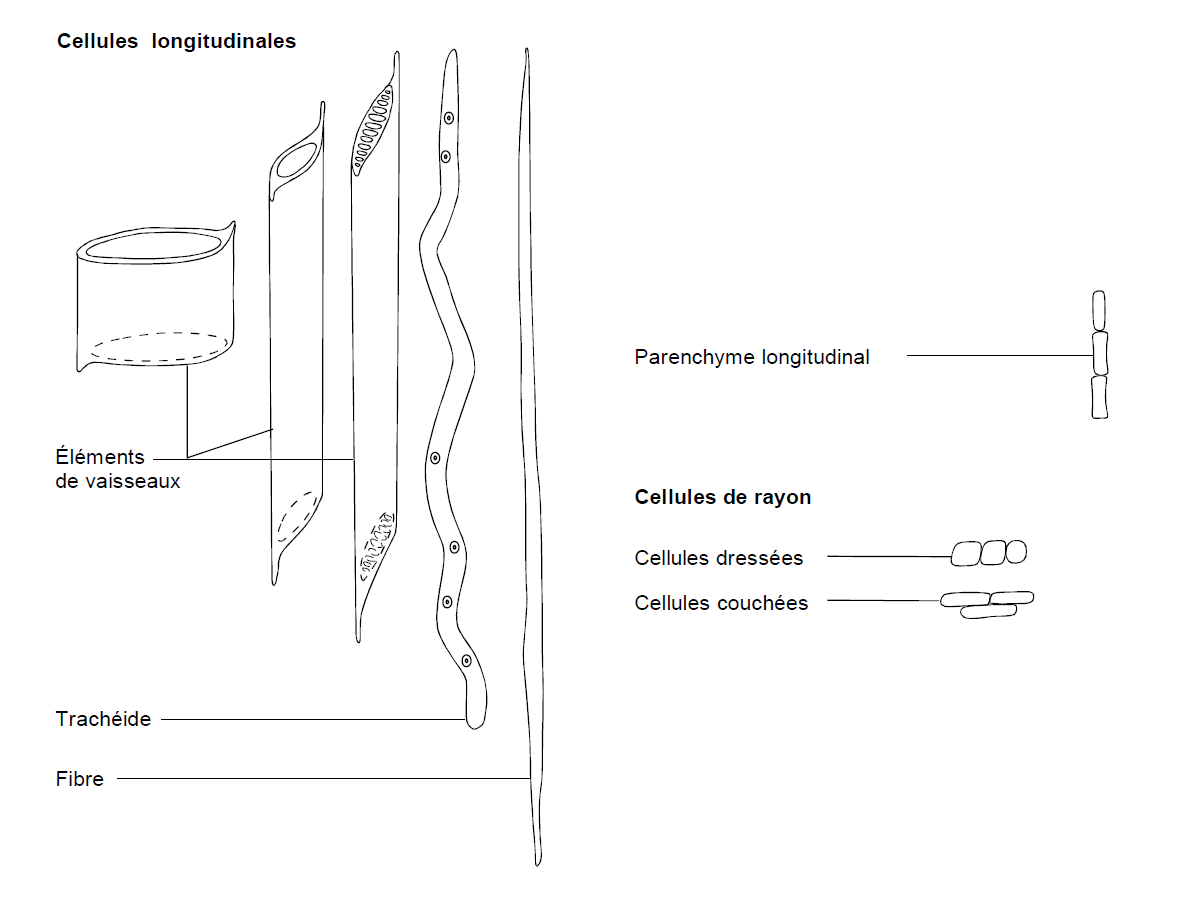
\includegraphics[scale=0.5]{img/ch4_type_cell}
\caption{Forme et longueur relative des principaux types de cellules des bois feuillus (adapté de \cite{hoadley1990identifying})}
\label{fig:ch4_type_cell}
\end{figure}

\begin{figure}[h]
\centering
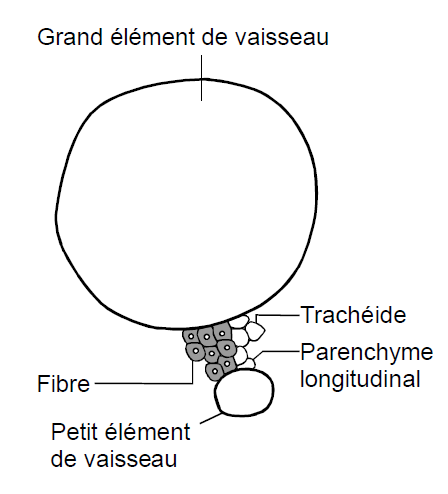
\includegraphics[scale=0.5]{img/ch4_form_cell_X}
\caption{Forme, diamètre et épaisseur des parois cellulaires relatives des principaux types de cellules des bois feuillus (adapté de \cite{hoadley1990identifying})}
\label{fig:ch4_form_cell_X}
\end{figure}

\section{Cellules orientées longitudinalement}

On peut séparer les cellules orientées longitudinalement en deux grands groupes : les éléments de vaisseaux (trachéides et fibres) et le parenchyme longitudinal.

\begin{description}
\item[Éléments de vaisseaux (trachéides et fibres)] Il s'agit de cellules allongées possédant une variété de types de ponctuations et servant à la conduction de la sève brute et au support mécanique de la tige. Ces cellules perdent leur protoplasme aussitôt qu'elles ont atteint leur maturité à partir des initiales fusiformes du cambium.

\item[Parenchyme longitudinal] Ces cellules conservent leur protoplasme dans l'aubier. Ce sont des cellules courtes possédant des ponctuations simples et servant à l'entreposage des substances nutritives.
\end{description}

\subsection{Éléments de vaisseaux}

Les éléments de vaisseaux sont les unités de base formant les structures composites en forme de tubes que l'on appelle vaisseaux ou pores.  Les éléments de vaisseaux sont les cellules des bois feuillus possédant les plus grands diamètres mais aussi une paroi cellulaire mince.  Ils sont disposés les uns sur les autres en séries verticales et leurs parois terminales sont perforées de façon à former un tube continu permettant le passage des fluides, c'est-à-dire un vaisseau. Les parois terminales sont perforées par action enzymatique avant que le protoplasme ne soit éliminé.  Cette opération produit ce qu'on appelle les cloisons perforées qui ont des formes différentes en fonction des espèces.\\

Les vaisseaux ne sont pas des tubes verticaux rectilignes indépendants les uns des autres. Au contraire, les vaisseaux dévient par rapport à la verticale et ce jusqu'à 30 cm par 5 m de longueur.  De plus, ils sont interconnectés par des ponctuations et cloisons perforées de façon à créer un réseau de pores permettant d'éviter les cul-de-sacs.\\

La longueur des éléments de vaisseaux varie considérablement en fonction des espèces (Tableau~\ref{tab:long_vaiss}) même si peu ou pas de croissance en longueur ne se produit pour ces cellules. Ceci est dû au fait que la longueur des initiales fusiformes du cambium varie d'une espèce à l'autre (0,18 à 1,3 mm).  On remarque que la longueur des éléments de vaisseaux varie d'environ 0,22 à 1,00 mm alors que celle des fibres varie d'environ 0,9 à 1,55 mm pour les principales espèces de feuillus de l'Est de l'Amérique du Nord.\\

Quant au diamètre des vaisseaux ou pores, il est mesuré selon la direction tangentielle et varie de 20 \micro m jusqu'à 300 \micro m en fonction des espèces.

\begin{table}[ht]
	\centering
	\begin{tabular}{l c c c c}
		\hline
		\bf Espèce & \multicolumn{2}{c}{\textbf{Éléments de vaisseaux}} & \multicolumn{2}{c}{\textbf{Fibres}}\\
		& \bf long. moy. (mm) & \bf Écart-type & \bf long. moy. (mm) & \bf Écart-type \\
		\hline
		\hline
		Érable à sucre	&	0,41	&	0,09	&	0,92	&	0,13	\\
		Bouleau jaune	&	0,84	&	0,16	&	1,38	&	0,17	\\
		Bouleau à papier	&	1,00	&	0,26	&	1,35	&	0,15	\\
		Frêne blanc	&	0,29	&	0,03	&	1,26	&	0,17	\\
		Frêne noir	&	0,27	&	0,04	&	1,27	&	0,17	\\
		Noyer cendré	&	0,36	&	0,14	&	1,13	&	0,17	\\
		Noyer noir	&	0,51	&	0,08	&	1,21	&	0,14	\\
		P. faux-tremble	&	0,67	&	0,18	&	1,32	&	0,22	\\
		Chêne rouge	&	0,42	&	0,09	&	1,32	&	0,29	\\
		Orme d’Amérique	&	0,22	&	0,04	&	1,55	&	0,20	\\
		\hline
	\end{tabular}
	\caption{Longueur des éléments de vaisseaux et des fibres des principales espèces de feuillus de l'est de l'Amérique du Nord.}\label{tab:long_vaiss}
\end{table}

\subsubsection{Disposition des vaisseaux}

On peut classer les bois feuillus en trois grands groupes en fonction de la disposition et de la taille des vaisseaux.  Ces critères constituent en fait la première étape dans l'identification des bois feuillus. Ces trois groupes sont illustrés à la figure~\ref{fig:dispo_pores} et décrits ci-dessous.

\begin{description}

\item[Bois à zone poreuse] Les vaisseaux formés au printemps ont un diamètre beaucoup plus grand que ceux formés plus tard en saison. On peut rencontrer une ou plusieurs rangées de gros vaisseaux formant le bois initial.  Les chênes, ormes et frênes sont caractéristiques des bois à zone poreuse.

\item[Bois à zone semi-poreuse] Les vaisseaux formés au printemps ont un diamètre maximum et ce diamètre diminue et demeure constant ou continue à diminuer dans le cerne annuel. Les noyers (\textit{Juglans spp.}) sont caractéristiques des bois à zone semi-poreuse.

\item[Bois à pores diffus] Les vaisseaux ont un diamètre plutôt constant et sont répartis uniformément dans le cerne annuel. Les érables (\textit{Acer spp.}), bouleaux (\textit{Betula spp.}), hêtres (\textit{Fagus spp.}) et tilleuls (\textit{Tilia spp.}) sont caractéristiques des bois à pores diffus.
\end{description}

\begin{figure}[h]
\centering
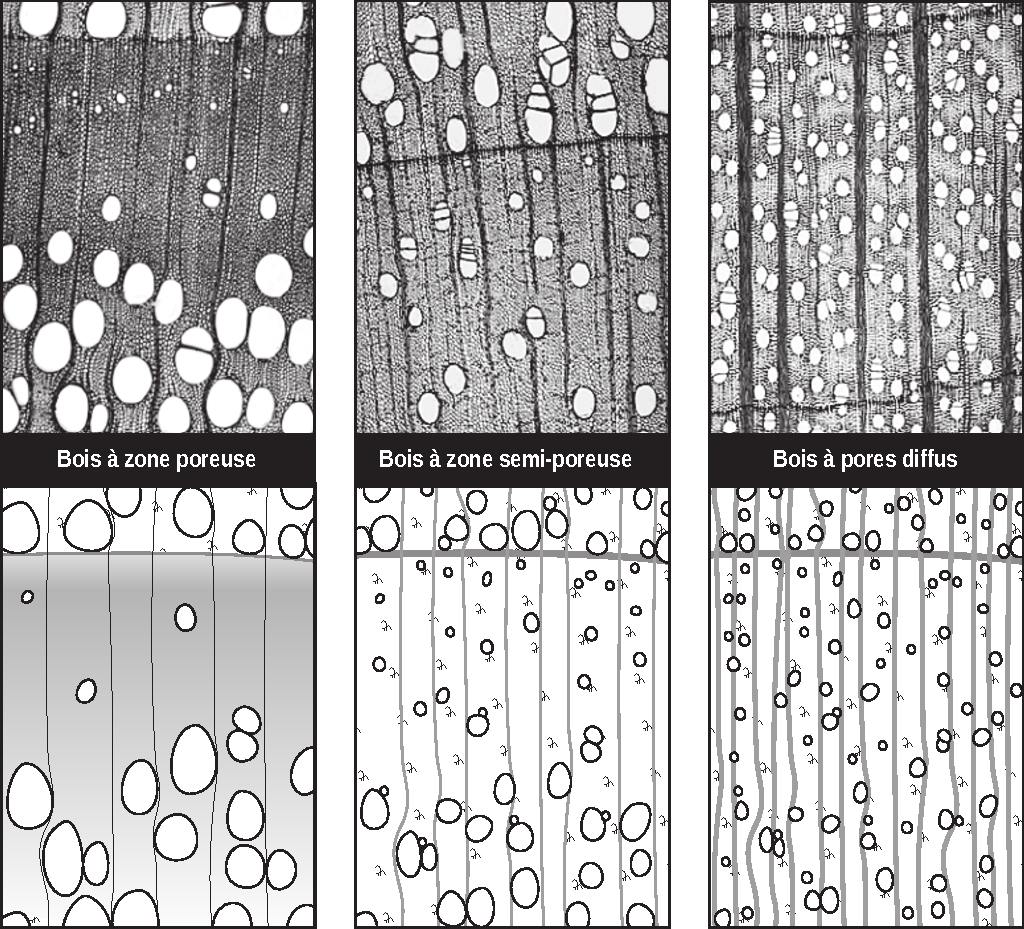
\includegraphics[scale=0.6]{img/ch4_dispositon_pores}
\caption{Disposition des pores chez les feuillus. Image préparée par Julie Ferland pour \cite{achim2010dendroecologie}.}
\label{fig:dispo_pores}
\end{figure}

\subsubsection{Caractéristiques des éléments de vaisseaux}

Certaines caractéristiques des éléments de vaisseaux sont utilisées pour l'identification des bois feuillus.  Il s'agit 1) de la forme des cloisons perforées, 2) de la disposition des ponctuations intervasculaires et 3) de la présence d'épaississements spiralés.

\subsubsection{Forme des cloisons perforées}\label{cloisons}

Les cloisons perforées sont les ouvertures que l'on retrouve dans la paroi commune entre deux éléments de vaisseaux.  On retrouve habituellement deux cloisons perforées par élément de vaisseau mais il peut y en avoir davantage pour permettre l'interconnexion entre les vaisseaux. On trouve plusieurs types de cloisons perforées:

\begin{description}
\item[Perforation unique (\textit{simple})] La perforation unique consiste en une ouverture simple occupant habituellement toute la surface de la cloison perforée (Figure~\ref{fig:cloisons}). On retrouve ce type de perforation chez environ 80\% des feuillus d'Amérique du Nord. On nomme bourrelet de la perforation le résidu de la paroi cellulaire perforée qui forme un anneau autour d'une perforation unique.

\begin{figure}[h]
	\centering
	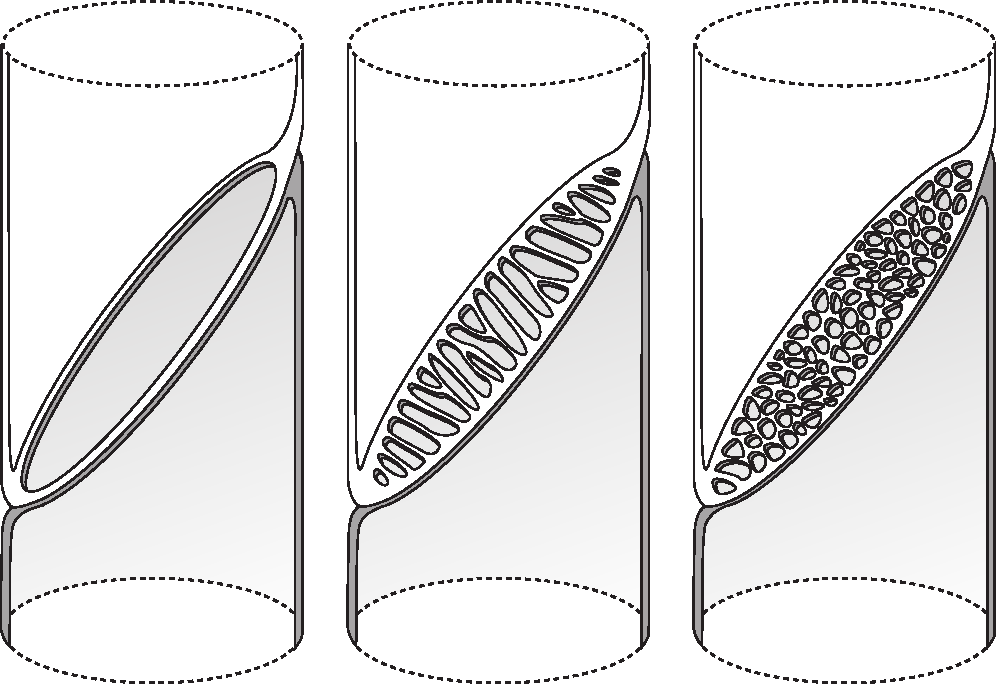
\includegraphics[scale=0.6]{img/ch4_perforation_cloison}
	\caption{Cloisons perforées chez les éléments de vaisseaux.  a) perforation unique; b) perforation en grille; c) perforation en réseau. Image préparée par Julie Ferland pour \cite{achim2010dendroecologie}.}
	\label{fig:cloisons}
\end{figure}

\item[Perforation en grille (\textit{scalariform})] La perforation en grille consiste en une série d'ouvertures parallèles orientées transversalement (Figure~\ref{fig:cloisons}). Les résidus de la paroi cellulaire demeurant dans la cloison perforée ont l'apparence des barreaux d'une échelle (Figure~\ref{fig:grille}) d'où le nom anglais \og scalariform \fg. Elles sont typiques chez les bouleaux (\textit{Betula spp.}). Le nombre de barreaux varie d'une espèce à l'autre.  On peut retrouver les deux types de perforation, unique et en grille, chez certaines espèces (ex. : hêtre à grandes feuilles (\textit{Fagus grandifolia})).

\item[Perforation en réseau (\textit{reticulate})] La perforation en réseau est semblable à la perforation en grille sauf que les résidus de la paroi cellulaire encore présents dans la cloison perforée ont l'apparence d'un filet plutôt irrégulier (Figures~\ref{fig:cloisons}~et~\ref{fig:reseau}). Ce type de perforation n'est toutefois pas présent chez les espèces commerciales de l'Amérique du Nord.
\end{description}

\begin{figure}[h]
\centering
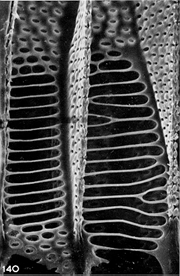
\includegraphics[scale=1]{img/ch4_grille}
\caption{Perforation en grille chez Alnus glutinosa (d'après \cite{butterfield2012three})}
\label{fig:grille}
\end{figure}

\begin{figure}[h]
\centering
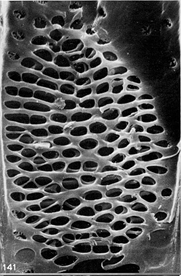
\includegraphics[scale=1]{img/ch4_reseau}
\caption{Perforation en réseau chez \textit{Coprosma tenuicaulis} (d'après \cite{butterfield2012three})}
\label{fig:reseau}
\end{figure}

\subsubsection{Disposition des ponctuations intervasculaires}\label{disposition}

Tout comme c'est le cas chez les résineux, le type de ponctuations que l'on retrouve entre les cellules des bois feuillus dépend du type de cellules en contact entre elles.  Il faut noter en particulier que les parois des cellules de parenchyme des feuillus sont plus épaisses que celles des résineux. Il s'agit de parois primaires \og épaissies \fg pouvant donner des couples de ponctuations aréolées ou semi-aréolées. Il faut remarquer que chez les feuillus, les couples de ponctuations aréolées ne comportent pas de torus comme chez les conifères.\\

On peut donc avoir les types de ponctuation suivants en fonction du type de cellules en cause (Figure~\ref{fig:type_ponct_feuillus}).

\begin{figure}[h]
	\centering
	
	\begin{tikzpicture}[level distance=2.25in,sibling distance=.2in,scale=.75]
	\tikzset{edge from parent/.style= 
		{thick, draw,
			edge from parent fork right},every tree node/.style={draw,minimum width=1in,text width=1.5in, align=center},grow'=right}
	\Tree 
	[. {Élément de vaisseau}
		[.{Élément de vaisseau}
			[.{En file obliques (alternate)} ]
			[.{En rangées horizontales (opposite)} ]
			[.{En disposition scalariforme (scalariform)} ]
		]
		[.{Cellule de parenchyme}
			[.{Aréolées} ]
			[.{Semi-aréolé} ]
			[.{Simples} ]
		] 
		[. {Fibre ou trachéide}
			[.{Aréolées} ]
			[.{Rangées verticales} ]
		] 
	]
	\end{tikzpicture}
	\caption{Types de ponctuations entre les éléments de vaisseaux et chacun des types de cellules du bois des feuillus}
\label{fig:type_ponct_feuillus}	
\end{figure}

Les ponctuations intervasculaires sont celles que l'on retrouve sur les parois des éléments de vaisseaux, particulièrement en plan longitudinal-tangentiel. Elles servent au passage de la sève brute d'un vaisseau à l'autre. Il s'agit de couples de ponctuations aréolées.  On reconnaît trois types de disposition des ponctuations intervasculaires : 1) les ponctuations intervasculaires en files obliques, 2) les ponctuations intervasculaires en rangées horizontales et 3) les ponctuations intervasculaires en disposition scalariforme. Les trois types sont illustrés à la Figure~\ref{fig:intervasc}.


\begin{figure}[h]
\centering
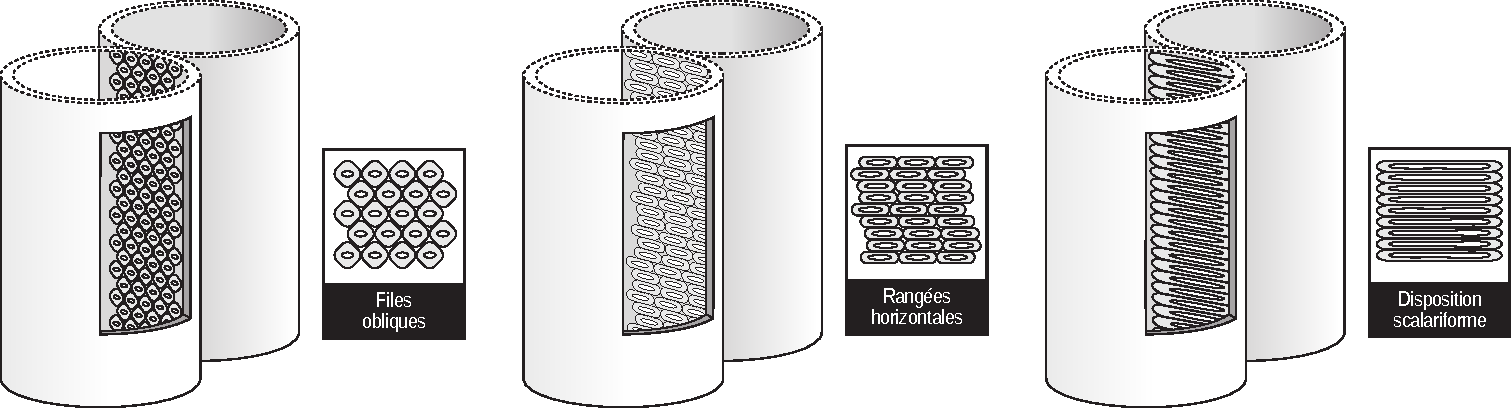
\includegraphics[scale=0.55]{img/ch4_ponctuations_intervasculaires}
\caption{Disposition des ponctuations intervasculaires. Image préparée par Julie Ferland pour \cite{achim2010dendroecologie}.}
\label{fig:intervasc}
\end{figure}	

Les ponctuations intervasculaires peuvent être classées selon leur dimension:

\begin{itemize}
\item diamètre de 2 à 4 \micro m:	petites (\textit{Betula spp.})
\item diamètre de 5 à 10 \micro m:	moyennes (\textit{Acer spp.})
\item diamètre de 12 à 50 \micro m:	grandes (\textit{Magnolia spp.})
\end{itemize}

\subsubsection{Épaississements spiralés dans les éléments de vaisseaux}\label{epais}

Des épaississements peuvent être présents dans la paroi secondaire des éléments de vaisseaux, des fibres et des trachéides chez certaines espèces et ils servent de critère d'identification. Ils sont des épaississements de la couche \hyperref[s3]{S\sub{3}} de la paroi cellulaire (voir chapitre~\ref{paroi}). Chez les bois à pores diffus, lorsque les épaississements spiralés sont présents, ils le sont pour tous les vaisseaux du cerne annuel. Chez les bois à zone poreuse, lorsqu'ils sont présents, on ne retrouve les épaississements spiralés  que chez les plus petits vaisseaux du bois final (Figure~\ref{vaiss_spiral}). Les épaississements spiralés dans les vaisseaux sont caractéristiques des érables (\textit{Acer spp.}), du cerisier tardif (\textit{Prunus serotina}) et du tilleul d'Amérique (\textit{Tilia americana}). On retrouve des épaississements spiralés dans les trachéides vasculaires chez l'orme rouge (\textit{Ulmus rubra}).

\begin{figure}[h]
\centering
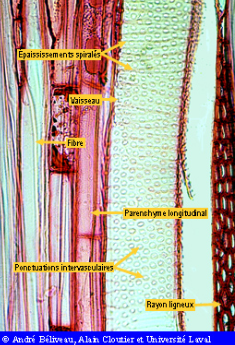
\includegraphics[scale=0.8]{img/ch4_vaiss_spiral}
\caption{Épaississements spiralés dans un vaisseau de tilleul d'Amérique (\textit{Tilia americana}) (grossissement $\times$400).}
\label{vaiss_spiral}
\end{figure}

\subsubsection{Incrustations dans les éléments de vaisseaux}

Un thylle (tylosis) est une excroissance d'un parenchyme adjacent dans un vaisseau, à travers une ponctuation. Les thylles peuvent obstruer un vaisseau ou le bloquer complètement si ils sont suffisamment nombreux. Les thylles sont généralement formés dans la partie intérieure de l'aubier, juste avant que la duraminisation se produise.  Ils peuvent parfois se former au début de l'aubier s'il y a sécheresse, blessure ou infection. On parle alors de thylles traumatiques. Le chêne blanc (\textit{Quercus alba}) est une espèce caractéristique présentant de nombreux thylles. Des thylles caractéristiques sont présentés à la Figure~\ref{fig:thylles}. \\

\begin{figure}[h]
	\centering
	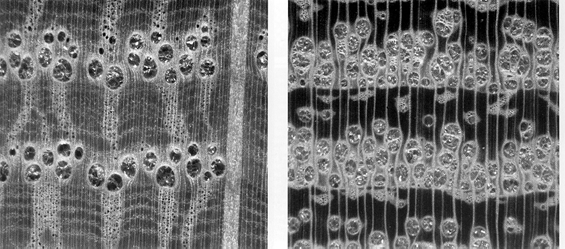
\includegraphics[scale=0.6]{img/ch4_thylles}
	\caption{Thylles dans les vaisseaux du chêne blanc (\textit{Quercus alba}) (à gauche) et de l'acacia blanc (Robinia pseudoacacia) (à droite) (grossissement: $\times$20) (d'après \cite{hoadley1990identifying})}
\label{fig:thylles}
\end{figure}

Des gommes et des résines peuvent aussi être sécrétées dans les vaisseaux.  Ces substances proviennent souvent des parenchymes de rayon et s'écoulent dans les vaisseaux par les ponctuations que l'on retrouve entre les vaisseaux et les parenchymes de rayon.  Elles sont caractéristiques de quelques espèces d'Amérique du Nord, par exemple le cerisier tardif (\textit{Prunus serotina}).

\subsubsection{Volume des vaisseaux}

Les vaisseaux constituent en moyenne 30\% du volume des bois feuillus, mais avec une variabilité importante entre les espèces (de 7 à 55\%). Chez les bois feuillus d'Amérique du Nord, la moyenne est plutôt d'environ 20\% du volume. La proportion du volume du bois occupée par les diverses composantes est présentée au Tableau~\ref{tab:prop_feuillus}.

\begin{table}[ht]
\centering
	\begin{tabular}{l c c c c}
	\hline
		& \bf Vaisseaux	& \bf	Fibres	& \bf	Rayons	& \bf	Parenchyme longitudinal	\\
		\hline
		\hline
		Érable à sucre	&	21,0	&	61,0	&	17,9	&	0,1	\\
		Bouleau jaune	&	21,4	&	63,8	&	10,8	&	2,0	\\
		Bouleau à papier	&	10,6	&	75,7	&	11,7	&	2,0	\\
		Cerisier tardif	&	41,4	&	41,4	&	17,2	&	-	\\
		Frêne blanc	&	20,4	&	61,7	&	11,9	&	4,2	\\
		Frêne noir	&	11,6	&	69,4	&	12,0	&	7,0	\\
		Noyer cendré	&	22,6	&	58,0	&	10,4	&	9,0	\\
		Noyer noir	&	21,0	&	48,7	&	16,8	&	13,5	\\
		Chêne rouge	&	21,6	&	43,5	&	21,4	&	13,5	\\
		Orme d’Amérique	&	48,0	&	34,7	&	11,3	&	6,0	\\
	\hline
	\end{tabular}
\caption{Proportion (\%) du volume du bois occupé par ses diverses composantes.}
\label{tab:prop_feuillus}
\end{table}

\subsection{Trachéides}

\subsubsection{Trachéides vasculaires}

Les trachéides vasculaires ressemblent aux vaisseaux du bois final mais elles ne possèdent pas de cloison perforée dans les bouts (éléments de vaisseaux imparfaits). Elles sont associées à des vaisseaux, elles sont organisées en séries verticales (longitudinales) et possèdent des couples de ponctuations aréolées.  Elles peuvent avoir des épaississements spiralés et ont l'apparence de petits vaisseaux en coupe transversale.  Les trachéides vasculaires sont présentes chez les ormes (\textit{Ulmus spp.}) au voisinage des vaisseaux du bois final.

\subsubsection{Trachéides juxtavasculaires}

Les trachéides juxtavasculaires sont de courtes trachéides de forme irrégulière, se trouvant à proximité immédiate des vaisseaux et ne faisant pas partie d'une série axiale définie. Elles ne possèdent pas de cloison perforée dans les bouts mais possèdent un nombre important de couples de ponctuations aréolées et des parois minces. On les retrouve surtout autour des vaisseaux du bois initial et elles forment des zones irrégulières en forme de flammes en coupe longitudinale-radiale. On les retrouve, entre autres, chez les chênes (\textit{Quercus spp.}) et les frênes (\textit{Fraxinus spp.}).

\subsection{Fibres}

Les fibres sont de longues cellules de faible diamètre, possédant des parois cellulaires épaisses mais ne possédant pas de cloison perforée dans les bouts. On distingue deux types de fibres : les fibres-trachéides et les fibres ligneuses simpliciponctuées.

\subsubsection{Fibres-trachéides}

Les fibres-trachéides possèdent de nombreux couples de ponctuations aréolées habituellement faciles à observer au microscope optique.

\subsubsection{Fibres ligneuses simpliciponctuées}

Les fibres ligneuses simpliciponctuées  possèdent des ponctuations simples habituellement peu nombreuses ayant l'apparence de petites ouvertures circulaires souvent difficiles à voir au microscope optique. On peut retrouver un type de fibre ou l'autre ou bien les deux chez une espèce en particulier. Il est souvent difficile d'identifier le type de fibre avec certitude. \\

La proportion du volume total du bois occupé par les fibres-trachéides et les fibres ligneuses simpliciponctuées varie de 25\% à 75\% en fonction des espèces et en détermine largement la résistance mécanique.

\subsection{Parenchyme longitudinal}

Le parenchyme longitudinal est constitué de cellules courtes en forme de briques disposées en files longitudinales. Les cellules de parenchyme gardent longtemps leur protoplasme et restent physiologiquement actives. Leur rôle essentiel est la mise en réserve et la distribution de substances nutritives (hydrates de carbone). Pour cela, leur paroi est peu lignifiée et abondamment ponctuée. Leur activité cesse dans le bois de duramen. Ces cellules de parenchyme sont connectées entre elles par des ponctuations simples.\\

Chez les feuillus, le parenchyme longitudinal est disposé de façon particulière en fonction des espèces. Cette disposition caractéristique est utilisée comme critère d'identification. Le parenchyme longitudinal peut occuper une proportion importante du volume du bois en fonction des espèces. Cette proportion varie d'environ 1 à 25\% chez les espèces nord-américaines et peut aller jusqu'à 50\% chez certains feuillus tropicaux.\\

On reconnaît trois types de parenchyme longitudinal : 1) les files de cellules de parenchyme longitudinal, 2) les cellules de parenchyme fusiforme et 3) les cellules de parenchyme épithélial. Nous verrons chaque type dans les paragraphes qui suivent.

\subsubsection{Files de cellules de parenchyme longitudinal}

Les files de cellules de parenchyme longitudinal sont formées par divisions transversales de l'initiale fusiforme fille.  Elles consistent en des groupements de cellules pouvant varier de une à plusieurs et sont souvent visibles en coupe transversale. Leurs arrangements variables peuvent être utilisés pour l'identification. Classement du parenchyme longitudinal :

\begin{description}

\item[Parenchyme apotrachéal] Le parenchyme apotrachéal est typiquement isolé des vaisseaux. Le parenchyme apotrachéal peut être :

\begin{description}
	\item[dispersé] Le parenchyme apotrachéal dispersé est caractérisé par des cellules de parenchyme isolées en plan RT tel qu'illustré à la Figure~\ref{fig:parenchymes_feuillus}A.  Il est caractéristique des érables (\textit{Acer spp.}).
	
	\item[dispersé en chaînettes] Le parenchyme apotrachéal dispersé en chaînettes est caractérisé par des cellules de parenchyme regroupées en de courtes lignes tangentielles disposées entre les rayons en plan RT tel qu'illustré à la Figure~\ref{fig:parenchymes_feuillus}B.  Il est caractéristique des noyers (\textit{Juglans spp.}) et des tilleuls (\textit{Tilia spp.}).
	arenchyme apotrachéal terminal (ou marginal)

	\item[terminal] Le parenchyme apotrachéal est caractérisé par des cellules de parenchyme regroupées en couches plus ou moins larges à la fin du cerne annuel en plan RT tel qu’illustré à la Figure~\ref{fig:parenchymes_feuillus}C. Il est caractéristique des peupliers (\textit{Populus spp.}).
	
	\item[en couches] Le parenchyme apotrachéal en couches est caractérisé par des cellules de parenchyme regroupées en couches plus ou moins larges qui ne sont pas nécessairement localisées à la fin du cerne annuel en plan RT tel qu'illustré à la Figure~\ref{fig:parenchymes_feuillus}D. Il est caractéristique des caryers (\textit{Carya spp.}).
\end{description}

\item[Parenchyme paratrachéal] Le parenchyme paratrachéal est typiquement associé aux vaisseaux ou aux trachéides vasculaires. Il peut être :

\begin{description}
	\item[juxtavasculaire] Le parenchyme paratrachéal juxtavasculaire est caractérisé par quelques cellules de parenchyme disposées autour des vaisseaux mais ne les entourant pas complètement en plan RT tel qu'illustré à la Figure~\ref{fig:parenchymes_feuillus}E.  Il est caractéristique des érables (\textit{Acer spp.}).
	
	\item[circumvasculaire] Le parenchyme paratrachéal circumvasculaire est caractérisé par une ou plusieurs couches de cellules de parenchyme disposées autour des vaisseaux et les entourant complètement en plan RT tel qu'illustré à la Figure~\ref{fig:parenchymes_feuillus}F.  Il est caractéristique des frênes (\textit{Fraxinus spp.}).

	\item[aliforme] Le parenchyme paratrachéal aliforme est caractérisé par une ou plusieurs couches de cellules de parenchyme disposées autour des vaisseaux, les entourant complètement et s'étendant de chaque côté en forme d'aile en plan RT tel qu'illustré à la Figure~\ref{fig:parenchymes_feuillus}G. Il est caractéristique des frênes (\textit{Fraxinus spp.}).
	
	\item[anastomosé (confluent)] Le parenchyme paratrachéal anastomosé est caractérisé par une ou plusieurs couches de cellules de parenchyme disposées autour de plusieurs vaisseaux, les entourant complètement et formant des bandes irrégulières tangentielles en plan RT tel qu'illustré à la Figure~\ref{fig:parenchymes_feuillus}H. Il est caractéristique du \textit{Robinia pseudoacacia}.
	
	\item[en couche] Le parenchyme paratrachéal en couche est caractérisé par une ou plusieurs couches de cellules de parenchyme disposées autour de plusieurs vaisseaux, les entourant complètement et formant de larges bandes irrégulières tangentielles en plan RT tel qu'illustré à la Figure~\ref{fig:parenchymes_feuillus}I.  Il est caractéristique des caryers (\textit{Carya spp.}) et des hêtres (\textit{Fagus spp.}).
	
	\marginpar{Des parenchymes apotrachéals et paratrachéals peuvent être présents tous les deux chez la même espèce.}	
\end{description}

\end{description}

\begin{figure}[h]
\centering
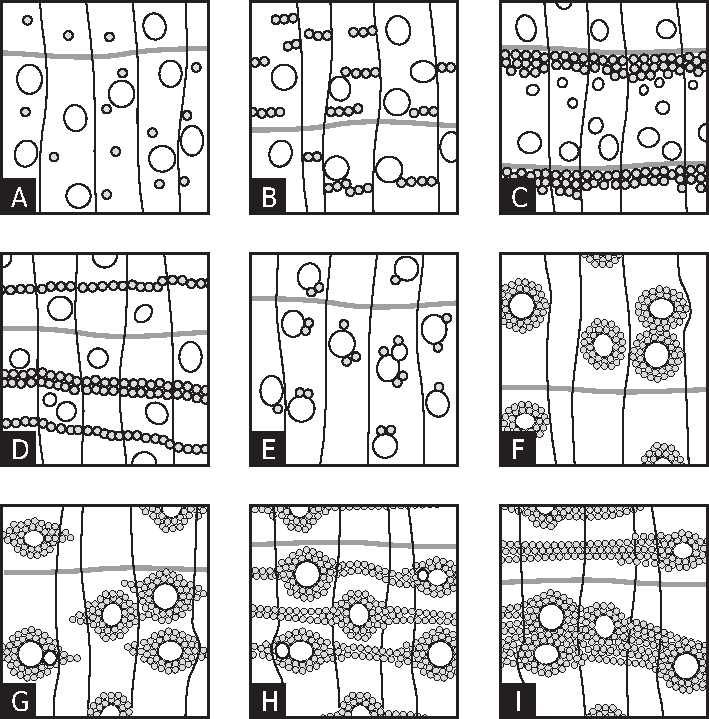
\includegraphics[scale=0.75]{img/ch4_parenchymes}
\caption{Différents types de parenchymes -- A. Dispersé B. Dispersé en chaînette C. Terminal D. En couche E. Juxtavasculaire F. Circumvasculaire G. Aliforme H. Anastomosé I. En couche}
\label{fig:parenchymes_feuillus}
\end{figure}

\subsubsection{Cellules de parenchyme fusiformes}

Le parenchyme fusiforme est un parenchyme longitudinal dérivé d'une initiale fusiforme sans subdivision.  Il s'agit donc d'une cellule de parenchyme allongée.  Ce type de parenchyme est rare chez les bois nord-américains.

\subsubsection{Cellules de parenchyme épithélial}

Les cellules de parenchyme épithélial tapissent les cavités des canaux longitudinaux (gomme ou résine) présents chez certains feuillus tropicaux.  Ces canaux sont absents chez les feuillus nord-américains.


\section{Cellules transversales}

Les cellules transversales constituent essentiellement les rayons comme c'est le cas chez les résineux. Les rayons présentent toutefois une plus grande variabilité chez les feuillus que chez les résineux à l'égard de la forme, de l'arrangement, de la largeur et de la hauteur.


\subsection{Composition des rayons}

Chez les feuillus, les rayons sont composés uniquement de cellules de parenchyme. Ces cellules sont de deux types: les cellules dressées et les cellules couchées. Les cellules dressées sont des cellules allongées verticalement et les cellules couchées sont des cellules allongées horizontalement.\\

On classe les rayons en deux catégories, les rayons homogènes et les rayons hétérogènes uniquement. Les rayons hétérogènes sont composés de cellules couchées et de cellules dressées (Figure~\ref{fig:rayons_feuillus}). Les rayons homogènes sont composés de cellules couchées ou de cellules dressées.

\begin{figure}[h]
\centering
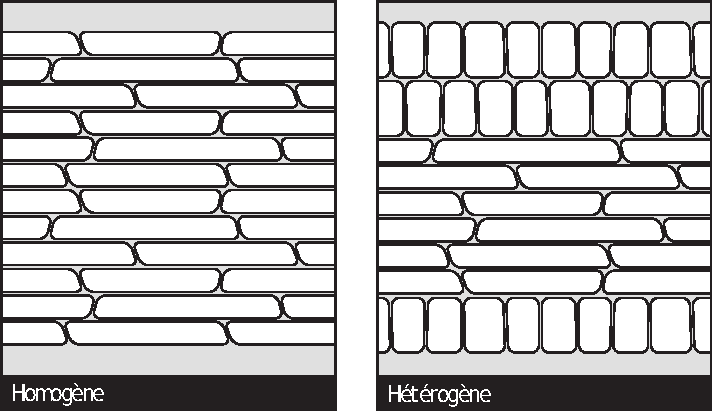
\includegraphics[scale=0.75]{img/ch4_rayons}
\caption{Différents types de rayons chez les feuillus (adapté de \cite{jane1970structure}).}
\label{fig:rayons_feuillus}
\end{figure}

\subsection{Taille des rayons}

Chez les feuillus, les rayons sont visibles ou non à l'oeil nu. Les peupliers (\textit{Populus spp.}) possèdent des rayons unisériés mais la plupart du temps, les rayons des feuillus sont plurisériés et ils peuvent être très larges comme chez les chênes (\textit{Quercus spp.}) où ils atteignent jusqu'à 30 cellules de large (30-sériés). Chez certaines espèces, les rayons sont de deux dimensions distinctes, soit des rayons unisériés et des rayons plurisériés. C'est le cas de l'érable à sucre (\textit{Acer saccharum}) et du hêtre à grandes feuilles (\textit{Fagus grandifolia}). La hauteur des rayons varie d'environ 20 m (une cellule) jusqu'à 50 mm.

\subsection{Espacement des rayons}

L'espacement des rayons est défini comme le nombre de rayons par millimètre en section transversale. Pour le déterminer, on mesure le nombre de rayons par mm traversant la fin ou le début du cerne annuel. Le classement de l'espacement des rayons est donné au Tableau~\ref{tab:espace_rayons}.

\begin{table}[ht]
	\centering
	\begin{tabular}{l l}
		\hline
		\bf Rayon/mm & \bf Espacement\\
		\hline
		\hline
		5 ou moins & Largement espacés\\
		6 à 9 & Normalement espacés \\
		10 à 13 & Plutôt rapprochés \\
		14 à 20 & Rapprochés \\
		21 ou plus & Extrêmement rapprochés\\
		\hline	
	\end{tabular}
	\caption{Classement de l'espacement des rayons}
\label{tab:espace_rayons}
\end{table}

\subsection{Ponctuations dans les rayons}

Les ponctuations des parenchymes de rayon vont de simples et petites à aréolées et grandes en fonction des cellules en contact avec les parenchymes de rayon. On reconnaît trois principaux types de ponctuations rayon-vaisseau:

\begin{enumerate}
\item Ponctuations rayon-vaisseau simples et allongées.
\item Ponctuations rayon-vaisseau simples à aréolées et variables en forme et en dimension.
\item Ponctuations rayon-vaisseau semblables aux ponctuations intervasculaires.
\end{enumerate}

\subsection{Contenus cellulaires}

Des contenus cellulaires sont souvent présents dans les cellules des rayons.  Il s'agit de cristaux, de silice, de substances amorphes (gommes, résines, tannins, huiles, latex, \ldots) ou d'amidon.

\subsection{Proportion des rayons}

La proportion du volume des bois feuillus constituée par des rayons varie de 10 à 20\%. La proportion en volume des rayons a un effet important sur les propriétés mécaniques du bois en termes de stabilité dimensionnelle, de formation de gerces et de fentes internes lors du séchage, de perméabilité et de résistance mécanique.

\subsection{Canaux à gomme}

Des canaux à gommes normaux ou traumatiques peuvent être présents. Ces canaux contiennent des cellules épithéliales sécrétant des gommes ou résines. Des canaux à gommes \og normaux \fg ne sont pas présents chez les espèces nord-américaines.

\section{L'anatomie du bois des feuillus en un clin d'œil}

La figure~\ref{fig:Fahn_feu} illustre l'organisation des différentes cellules du bois des résineux.

\begin{figure}[h]
\centering
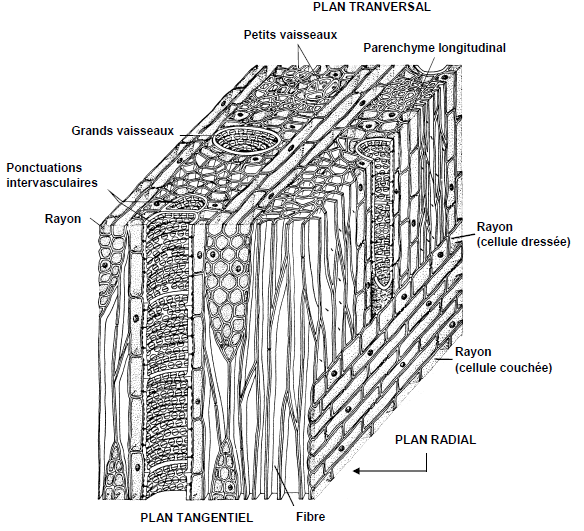
\includegraphics[scale=0.7]{img/ch4_Fahn_feu}
\caption{Structure tridimensionnelle générale des feuillus (adapté de \cite{fahn1990plant})}
\label{fig:Fahn_feu}
\end{figure}
%
%
%
%Références
%
%
%
%Butterfield, B.G.; Meylan, B.A. 1980. Three-dimensional structure of wood. An ultrastructural approach. Second edition. Chapman and Hall, London, New York. 103 p.
%
%Fahn, A. 1990. Plant anatomy. Fourth edition. Pergamon Press, Oxford. 588 p.
%
%Hoadley, R.B. 1990. Identifying wood. Accurate results with simple tools. The Taunton Press Inc. Connecticut, USA. 223 p.
%
%Jane, F.W. 1970. The structure of wood.  Second Edition.  Adam and Charles Black, London.  478 p.
%
%Panshin, A.J.; de Zeeuw, C. 1980. Textbook of wood technology. Fourth edition. McGraw-Hill Book Co. New York. 722 p.
%
